\documentclass[12pt]{article}

\usepackage[utf8]{inputenc}
\usepackage{latexsym,amsfonts,amssymb,amsthm,amsmath}
\usepackage{tikz}
\usepackage{stanli}
\usetikzlibrary{shapes,calc,through,3d,patterns}
\usetikzlibrary{arrows.meta,decorations.pathreplacing,angles,quotes}
\usepackage{multicol}
\usepackage{geometry}
\usepackage{mathtools}
\usepackage{siunitx}
\usepackage{booktabs}

\setlength{\parindent}{0in}
\setlength{\oddsidemargin}{-0.25in}
\setlength{\textwidth}{7in}
\setlength{\textheight}{9.3in}
\setlength{\topmargin}{-1in}
\setlength{\headheight}{18pt}

\newcommand\blfootnote[1]{%
    \begingroup
    \renewcommand\thefootnote{}\footnote{#1}%
    \addtocounter{footnote}{-1}%
    \endgroup
}

\definecolor{darkred}{rgb}{0.6,0,0}

\newcommand{\bolddelta}{\boldsymbol\delta}
\newcommand{\boldxi}{\boldsymbol\xi}

\begin{document}

\noindent ME473 - Dynamic finite element analysis of structures\hfill EPFL\\
Stefano Burzio \hfill 2025\\
\vspace{0.3cm}

\hspace*{\fill}\textbf{\Large Problem set 3 - solutions}\hspace*{\fill}

\hrulefill

\subsection*{Problem 1}
Assuming that the approximate longitudinal displacement \( u^h(x,t) \) can be expressed as
\[
    u^h(x,t) = h_1(x)q_1(t) + h_2(x)q_2(t) + h_3(x)q_3(t),
\]
where \( h_i(x) \) represent the quadratic shape functions and \( q_i(t) \) denote the unknown nodal displacements, the semi-discrete weak formulation is expressed as follows:
\begin{equation}\label{sdwf2}
    \mathbf{M} \ddot{\mathbf{q}}(t) + \mathbf{K} \mathbf{q}(t) = 0, \quad t \in]0,T[
\end{equation}
where $\mathbf{M}$ and $\mathbf{K}$ are the global mass and stiffness matrices and $\mathbf{q}(t)=\{q_1(t),q_2(t),q_3(t)\}^T$ is the unknown nodal displacement vector. The components of $\mathbf{M}$ and $\mathbf{K}$ can be specified as
\begin{align*}
    m_{ij} & = \int_{0}^{\ell} \rho A \ h_i \ h_j \, dx,                                                                                 \\
    k_{ij} & = \int_{0}^{\ell} EA \ \left( \frac{\partial h_i}{\partial x} \right) \left( \frac{\partial h_j}{\partial x} \right) \, dx,
\end{align*}
Note that the system of equations \eqref{sdwf2} will still need to be modified to include the homogenoeus boundary condition $q_1 = 0$.

Since the finite element $\Omega = ]0,\ell[$ is quadratic, the three global parabolic shape functions, which are linearly independent and satisfy the convergence criteria, are expressed as
\begin{align*}
    h_1(x) & =l_1[x_1,x_2,x_3](x)=\prod_{\substack{m=1 \\ m\neq 1}}^{3}\frac{x-x_m}{x_1-x_m} = 1 - \frac{3}{\ell}x + \frac{2}{\ell^2}x^2 \\
    h_2(x) & =l_2[x_1,x_2,x_3](x)=\prod_{\substack{m=1 \\ m\neq 2}}^{3}\frac{x-x_m}{x_2-x_m}= \frac{4}{\ell}x- \frac{4}{\ell^2}x^2                  \\
    h_3(x) & =l_3[x_1,x_2,x_3](x)=\prod_{\substack{m=1 \\ m\neq 3}}^{3}\frac{x-x_m}{x_3-x_m}= -\frac{1}{\ell}x + \frac{2}{\ell^2}x^2
\end{align*}\begin{center}
    \begin{tikzpicture}
        % Draw axes
        \draw[-latex] (-0.5, 0) -- (4.5, 0) node[right] {$x$};
        \draw[-latex] (0, -0.5) -- (0,2.5) node[above] {$y$};
        % Define points
        \coordinate (O) at (0, 0);
        \coordinate (A) at (2, 0);
        \coordinate (B) at (4, 0);
        \coordinate (H) at (2, 0);
        \coordinate (K) at (2, 2);
        \coordinate (J) at (4, 2);
        % Mark points
        \draw[ultra thick] (O) -- (B);
        \draw[ultra thin] (-.1,2) node[left] {$1$} -- (.1,2);
        \fill (O) circle (3pt) node[below right] {$x_{1}$};
        \fill (B) circle (3pt) node[below right] {$x_{3}$};
        \draw[fill=white, draw=black] (A) circle (3pt) node[below] {$x_{2}$};
        % Label the function
        \draw[thick, darkred,domain=0:4, smooth, variable=\x]
        plot ({\x}, {2*(1-3*\x/4+2*\x*\x/16)});
        \draw[thick, orange,domain=0:4, smooth, variable=\x]
        plot ({\x}, {2*(4*\x/4-4*\x*\x/16)});
        \draw[thick, brown,domain=0:4, smooth, variable=\x]
        plot ({\x}, {2*(-\x/4+2*\x*\x/16)});
        \node[darkred, above] at (0.6, 2) {$h_1(x)$};
        \node[orange, above] at (2, 2) {\small $h_2(x)$};
        \node[brown, above] at (3.4, 2) {\small $h_3(x)$};
        \draw [decorate,decoration={brace,amplitude=5pt,mirror,raise=4ex}]
        (O) -- (B) node[midway,yshift=-3em]{${}^{1}\Omega$};
    \end{tikzpicture}
\end{center}
Inserting these expressions into the coefficients $m_{ij}$ and $k_{ij}$ of the mass and stiffness matrices leads, after integration, to the system of equations:
\begin{equation}\label{system33}
    \frac{\rho A \ell}{30}
    \begin{bmatrix}
        4  & 2  & -1 \\
        2  & 16 & 2  \\
        -1 & 2  & 4
    \end{bmatrix}
    \ddot{\mathbf{q}}(t) +
    \frac{E A}{3\ell}
    \begin{bmatrix}
        7  & -8 & 1  \\
        -8 & 16 & -8 \\
        1  & -8 & 7
    \end{bmatrix}
    \mathbf{q}(t) = 0
\end{equation}
in which the homogeneous boundary condition (clamping) $q_1 = 0$ and its virtual equivalent one $\delta q_1 = 0$ must now be incorporated. It follows that the first equation of \eqref{system33} must be eliminated, so that the problem reduces to solving for the displacements $q_2 (t)$ and $q_3 (t)$ the reduced system:
\begin{equation*}
    \frac{\rho A \ell}{30}
    \begin{bmatrix}
        16 & 2 \\
        2  & 4
    \end{bmatrix}
    \begin{bmatrix}
        \ddot{q}_2 \\
        \ddot{q}_3
    \end{bmatrix}
    +
    \frac{E A}{3\ell}
    \begin{bmatrix}
        16 & -8 \\
        -8 & 7
    \end{bmatrix}
    \begin{bmatrix}
        q_2 \\
        q_3
    \end{bmatrix}
    =
    \begin{bmatrix}
        0 \\
        0
    \end{bmatrix}.
\end{equation*}
By assuming an harmonic solution of pulsation $\omega$, the above expression becomes:
\begin{equation*}
    \left( \frac{\omega^2 \rho A \ell}{30}
    \begin{bmatrix}
        16 & 2 \\
        2  & 4
    \end{bmatrix}
    -
    \frac{E A}{3\ell}
    \begin{bmatrix}
        16 & -8 \\
        -8 & 7
    \end{bmatrix}
    \right)
    \begin{bmatrix}
        p_2 \\
        p_3
    \end{bmatrix}
    =
    \begin{bmatrix}
        0 \\
        0
    \end{bmatrix}
\end{equation*}
where the coefficients $p_i$ $(i=2,3)$ are the amplitudes of the harmonic function at nodal points 2 and 3. The characteristic equation \footnote{Refer to the \texttt{MATLAB} code for a detailed calculation.} associated with
\begin{equation*}
    \omega^4 - \omega^2 \left( \frac{104E}{3\rho \ell^2} \right) + \frac{80E^2}{\rho^2 \ell^4} = 0
\end{equation*}
provides the following two solutions, which correspond to the approximate natural frequencies of the bar,
$$ \omega_1 = 1.577 \sqrt{\frac{E}{\rho \ell^2}} \qquad\text{and}\qquad \omega_2 = 5.673 \sqrt{\frac{E}{\rho \ell^2}}.$$
Let us note the excellent accuracy of the fundamental frequency, which deviates by only 0.4\% from the exact value. However, the relative error in the second calculated frequency is significantly higher, reaching 20\% compared to the exact result. This significant difference arises because the bar is discretized using a single finite element. The basis functions, which have a parabolic shape, are poorly suited for accurately representing the three-quarters sine wave corresponding to the second mode, while they are sufficiently capable of approximating the quarter sine wave reflecting the first mode.

Nevertheless, it can be shown that higher-order natural frequencies quickly converge to the exact values as the mesh refinement increases.

\subsection*{Problem 2}

Discretizing the weak form using the finite element procedure leads to the following system of equations:
\begin{equation}
    \label{sdwf3}
    \mathbf M\ddot{\mathbf q}(t)+\mathbf K\mathbf q(t)=\mathbf r(t)
\end{equation}
where the mass and stiffness matrices have components given by $(i, j=1,\dots, 9) $
\begin{equation*}
    \begin{aligned}
         & m_{i j}=\rho\int_0^{2}\int_0^{2} h_i(x,y) h_j(x,y) \, dx\, dy                             ,                                         \\
         & k_{i j}=S\int_0^{2}\int_0^{2} \partial_{x}h_{i}(x,y)\partial_{x}h_{j}(x,y)+\partial_{y}h_{i}(x,y)\partial_{y}h_{j}(x,y)\,  dx\, dy.
    \end{aligned}
\end{equation*}
Moreover the components of the vector of applied forces are
$$r_i(t)=\int_0^{2}\int_0^{2} h_i(x,y)p(x,y,t)\, dx\, dy.$$
Notice that, due to the vanishing boundary conditions on $\Gamma$, the vector of unknown nodal displacements $\mathbf{q}=\{q_1,\dots,q_9\}^T$ has only one non zero component $q_5$, representing the transveral displacement of the center of the membrane. Therefore the system \eqref{sdwf3} reduces to one single equation:
$$m_{55}\ddot{q}_5(t)+k_{55} q_5(t)= r_5(t)$$
coupled with the initial conditions $q_5(0)=\dot q_5(0)=0$.

The bilinear quadrilateral shape function $h_5$ is defined as follows:
$$h_5(x,y)=\begin{cases}
        xy         & 0\leq x,y\leq 1                                   \\
        (2-x)y     & 1\leq x\leq 2,     \                0\leq y\leq 1 \\
        x(2-y)     & 0\leq x\leq 1,\ \ \ 1\leq y\leq 2                 \\
        (2-x)(2-y) & \pi\leq x,y\leq 2,                                \\
    \end{cases}$$
The following code, available on the \texttt{MATLAB} drive, is used to calculate and to plot the time response of the geometric center of the membrane $q_5(t)$. We start by definig the physical parameters that describe the membrane's properties and the symolic variables.
\begin{verbatim}
clc; clear; close all;
%% Problem Parameters
% Membrane length in x and y directions (m)
l = 2;  
% Tension per unit length (N/m)
S = 1000;  
% Material density (kg/m^2)
rho = 1200; 
% Load amplitude (N/m^2)
A = 100;   
% Forcing frequency (rad/s)
omega_bar = 10*pi; 
    
% Define symbolic variables
syms x y t q(t)
\end{verbatim}
The forcing function ($p$) represents the time-dependent external force (pressure) applied to the membrane. This force will vary with time and cause the membrane to oscillate.
\begin{verbatim}
% Define forcing function
p = A*sin(omega_bar*t);
\end{verbatim}
The shape function ($h_5$) is a piecewise function that defines the displacement shape of the membrane as a function of spatial coordinates $x$ and $y$. The function is broken into four regions of the membrane, each with a different mathematical expression.
\begin{verbatim}
% Define shape function and plot it 
h_5=piecewise((x >= 0) & (x <= l/2) & (y >= 0) & (y <= l/2), x*y, ...
                    (x >= l/2) & (x <= l) & (y >= 0) & (y <= l/2), (2-x)*y, ...
                    (x >= 0) & (x <= l/2) & (y >=l/2) & (y <= l), x*(2-y),...
                    (x >= l/2) & (x <= l) & (y >=l/2) & (y <= l),(2-x)*(2-y));
    
figure;
fsurf(h_5, [0, 2, 0, 2])
xlabel('x')
ylabel('y')
zlabel('h_5(x,y)')
title('3D Plot of base function h_5')
grid on
\end{verbatim}
\begin{center}
    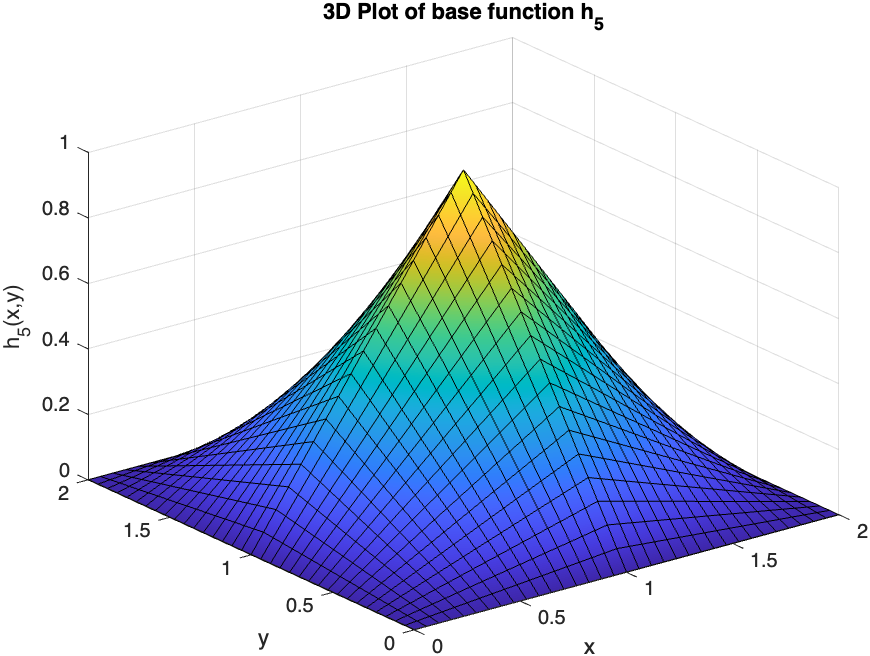
\includegraphics[width=8cm]{../images/h5plot.png}
\end{center}
\begin{verbatim}
   
% Compute the components of the stiffness and mass matrices and forces vector 
    
grad_h_5 = gradient(h_5, [x, y]);
    
k_55 = vpa(S * int(int(transpose(grad_h_5)*grad_h_5,x,[0,l]),y,[0,l]),4)
m_55 = vpa(rho * int(int(h_5^2,x,[0,l]),y,[0,l]),4)
r_5(t) = int(int(p*h_5,x,[0,l]),y,[0,l])
\end{verbatim}
Equation of motion (ODE): this is the core of the problem: the second-order ordinary differential equation (ODE) that describes the motion of the membrane over time. The displacement and the velocity at time $t=0$ is assumed to be zero. This represents the initial rest state of the membrane.

Solving the ODE: dsolve: This command solves the ODE symbolically to find the displacement  of the membrane as a function of time.
\begin{verbatim} 
% Define the ODE resulting form the discretization and solve it to find the
% time response at the node x_5
ode = m_55 * diff(q, t, 2) + k_55 * q == r_5(t);
initial_cond = [q(0) == 0, subs(diff(q, t), t, 0) == 0];
q_5 = dsolve(ode, initial_cond);
    
fplot(q_5,[0,10],'Linewidth',2);
xlabel('Time (seconds)')
ylabel('q_5(t) (meters)')
grid on    
\end{verbatim}
\begin{center}
    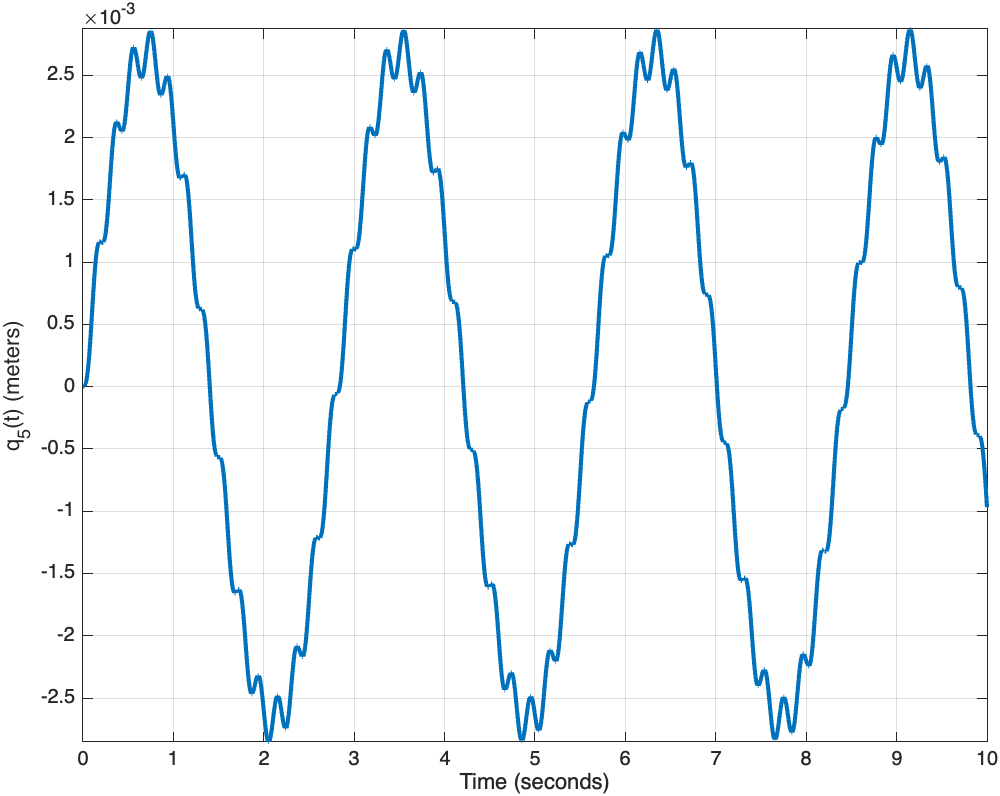
\includegraphics[width=8cm]{../images/q5plot.png}
\end{center}

\textbf{Resonance input frequency}
Resonance arises when the excitation frequency matches the fundamental natural frequency of the plate.
\begin{verbatim}
omega_fund_freq = sqrt(k_55 / m_55);

p_resonance = A*sin(omega_fund_freq*t);

r_5_resonance(t) = int(int(p_resonance*h_5,x,[0,l]),y,[0,l]);

% Define the ODE resulting form the discretization and solve it to find the
% time response at the node x_5
ode_resonance = m_55 * diff(q, t, 2) + k_55 * q == r_5_resonance(t);
initial_cond = [q(0) == 0, subs(diff(q, t), t, 0) == 0];
q_5_resonance = dsolve(ode_resonance, initial_cond);

%plotting
fplot(q_5_resonance,[0,10],'Linewidth',2);
xlabel('Time (seconds)')
ylabel('q_5(t) (meters)')
grid on
\end{verbatim}
\begin{center}
    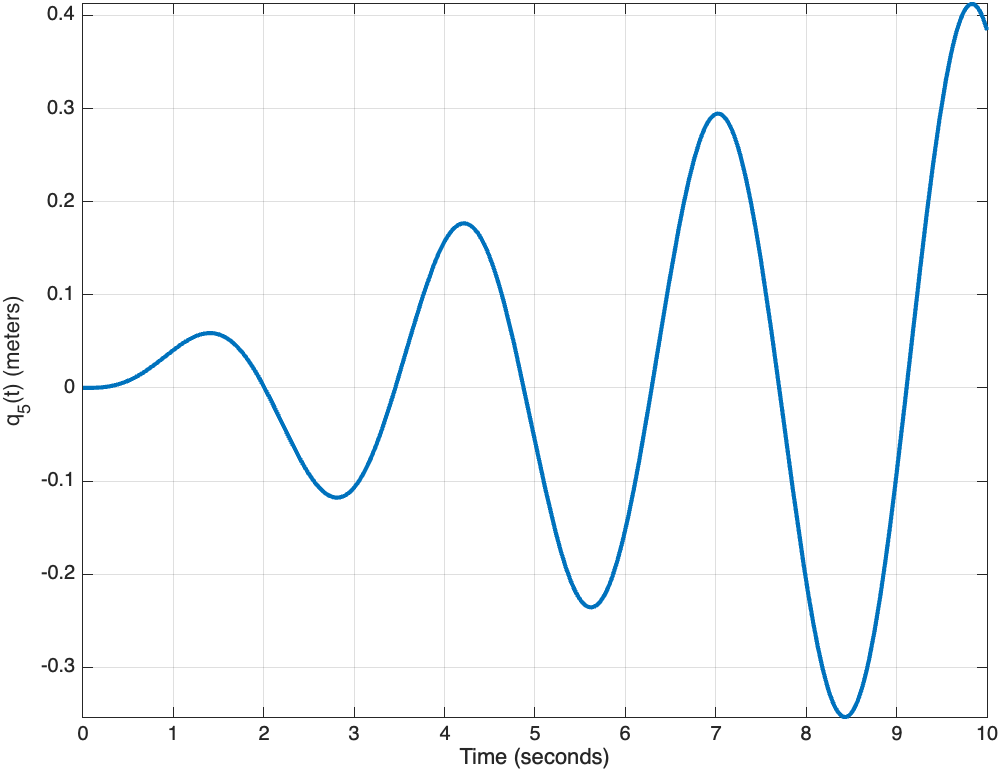
\includegraphics[width=8cm]{../images/q5plot_resonance.png}
\end{center}
\end{document}